\documentclass{article}
\usepackage{graphicx}

\begin{document}

\title{Using Structure Tensors to Find Beta Sheets in Protein Volume Images - An Implementation of Yu \& Bajaj's 2007 Technique}
\author{Jeff Donner}

\maketitle

\section{Overview}

It is possible to get 3D volume images of protein density, via
methods which are outside the scope of this paper. One helpful way to
\emph{identify} arbitrary proteins, is to take a mathematical signature
and compare them against a database of similarly derived signatures,
to at least narrow down the search for what known proteins the new one
might be. The two most prominent structures (known as \emph{secondary structures}
within proteins are, alpha helices and beta sheets. Alpha helices are
usually medium-to-long straight cylinders of fixed thickness (5 Angstroms).
Beta sheets are much less well-defined in shape, including curving, to almost
back on themselves. The one thing that is constant is that they are locally
flat, and within a certain range of thickness (something like 3.5 Angstroms).
This program implements Yu \& Bajaj's method \cite{yubajaj} of using the \emph{local structure
tensor} to detect and find the bounds of beta sheets.

\section{Technique and Algorithm}

The \emph{structure tensor} is an extension of the Principle Components Analysis (PCA) idea.
We might try to get the principal components \emph{of the gradient}, ie the shape, from the \emph{gradient tensor},
all pairwise products of $x, y, z$ directional derivatives

\[
  G =
\left( \begin{array}{ccc}
  f_{x}^2 & f_{x}f_{y} & f_{x}f_{z} \\
  f_{x}f_{y} & f_{y}^2 & f_{y}f_{z} \\
  f_{x}f_{z} & f_{y}f_{z} & f_{z}^2
\end{array} \right)
\]

and then take the eigenvalues and eigenvectors from this. But, this
produces only a single non-zero eigenvector, the net gradient. We want
the other two components as well, so we bring in 'influence' from the
gradients of neighboring voxels, so that the tensor contains
information that reflects a wider area. And, this will also produce up
to 3 eigenvectors when analysed. We gather this 'influence' by convolving
with a Gaussian function, $g_{\alpha}$, resulting in the \emph{structure tensor}

\[
  T_{\alpha} =
\left( \begin{array}{ccc}
  f_{x}^2*g_{\alpha} & f_{x}f_{y}*g_{\alpha} & f_{x}f_{z}*g_{\alpha} \\
  f_{x}f_{y}*g_{\alpha} & f_{y}^2*g_{\alpha} & f_{y}f_{z}*g_{\alpha} \\
  f_{x}f_{z}*g_{\alpha} & f_{y}f_{z}*g_{\alpha} & f_{z}^2*g_{\alpha}
\end{array} \right)
\]


The relative sizes of the eigenvalues indicate the local shape:
\begin{center}
  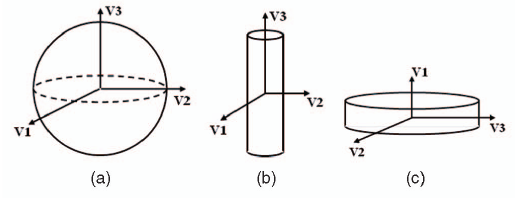
\includegraphics[width=60mm]{shapes.png}
\end{center}

Here $v_1$ is the direction of greatest gradient, that is, the density drops off quickest
in that direction, followed by $v_2$, $v_3$.

The algorithm runs as follows:

We start with local density maxima (these points will be usually
within alpha helices or beta sheets), then see whether the local
structure is characteristic of a beta sheet. This much had been done
previously, what was new with this paper is actually \emph{finding the
length of probable beta thickness} along the eigenvectors. This is
necessary because other, less-dense structures such as coils and
turns, show similar curved, flattish local structure, but beta sheets
can be distinguished from them by their thickness.

If a point is found likely to be within a beta sheet, we take a plane
perpendicular to the predominant eigenvector, intersect it with a small
cube around the data point, and use the intersections with the edges
as new candidates for being a beta point, thus exploring away from each seed.

\begin{center}
  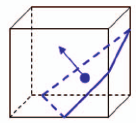
\includegraphics[width=20mm]{cube-plane.png}
\end{center}

When there are no more points to be explored, a triangle mesh is generated
from the intersecting polygons, and those comprise the 'beta signature'
of the protein.


%%  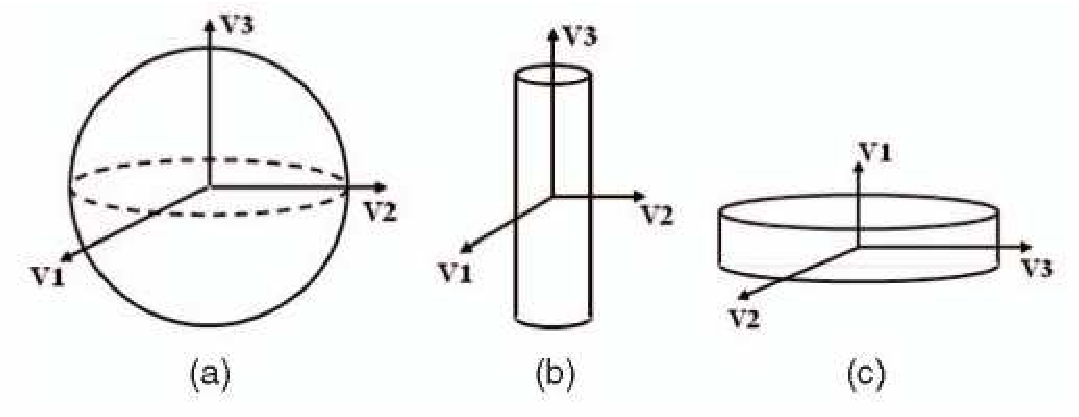
\includegraphics{shapes.pdf}
%%  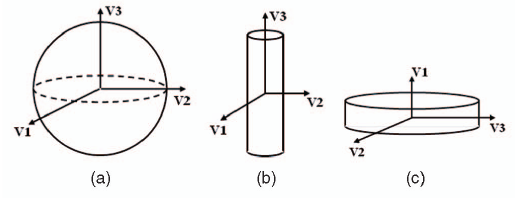
\includegraphics[height=60mm]{shapes.png}
%%  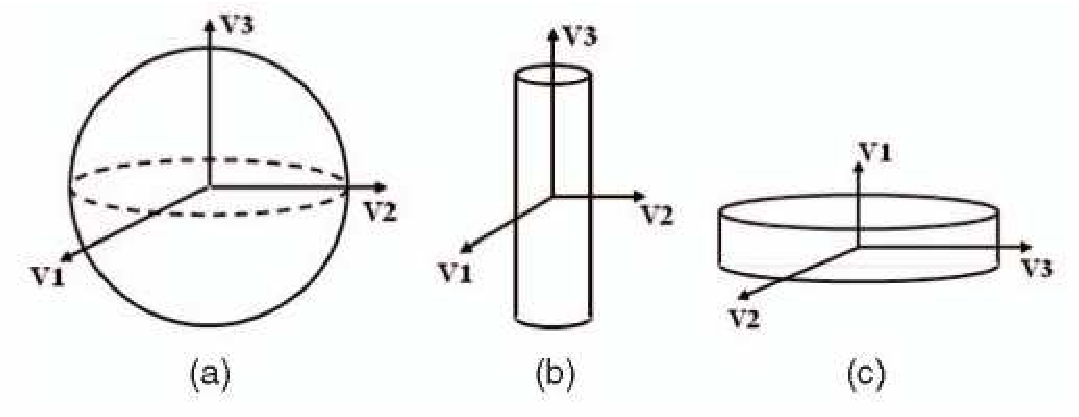
\includegraphics[scale=0.75]{shapes.pdf}
%%  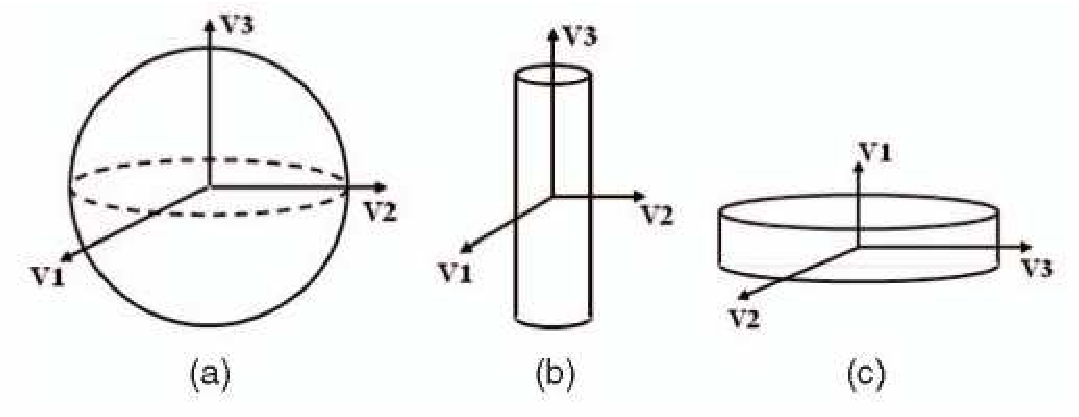
\includegraphics[angle=45,width=52mm]{shapes.jpg}


\section{Programming Decisions}

ITK \cite{itk} was chosen because it is pre-made for medical image
processing, and has much of what this project needed. It required time
to absorb, and the math and methods that it uses are obscured by being
abstracted across many layers (ie well-designed from a software
engineering standpoint!), but, the author would consider it first,
again, for similar projects. Only the gradient tensor and structure
tensors themselves were not already present, but they were
constructible from other ITK parts without great difficulty.


\section{Technical Description}

As mentioned, we use ITK, a powerful, free medical imaging toolkit.
ITK's architecture is to use image processing \emph{filter}s in which you hook
later stages up to earlier stages. There's also a lot of other functionality for things this framework doesn't apply to.

We wrote an .mrc ITK IO file filter, because the only tool we have to
generate volumes from protein description files (.pdb)
(pdb2mrc, part of the EMAN package)
produces the .mrc format.

Our use is: First the
\begin{enumerate}
\item Mrc format reader. This was added to our own local version of ITK (not submitted to the toolkit yet, though that is planned.)
\item We find local maxima ourselves (ITK has added this functionality since the project started, but we've continued to use our hand-made version).
\item Per the algorithm, we do a breadth-first search (this was a choice,
it could have been depth-first) on each of the seeds for its fit as a beta point,
per the equations above. We do this with ITK, a series of filters. For each
candidate point, we:
  \item Find its physical coordinates. Create a chunk of volume resampled
  around it, to support the Gaussian operations that come later.
  (This, because these operations operate on centered pixels, and later
  coordinates aren't exactly on data points, as the initial seeds are.
  Resampling makes a new volume, where the chosen coordinate and its neighbors,
  \emph{are} on data points.)
  \item Apply a derivative filter parallel to each axis (ITK's \texttt{DerivativeImageFilter}).
  We make an image rather than an single point from this, to give support
  to the Gaussian that we'll apply later.
  \item Cross-multiply these 3 images (by hand) to form
  \item the gradient tensor, where each point is a 9 element matrix

\[
  G =
\left( \begin{array}{ccc}
  f_{x}^2 & f_{x}f_{y} & f_{x}f_{z} \\
  f_{x}f_{y} & f_{y}^2 & f_{y}f_{z} \\
  f_{x}f_{z} & f_{y}f_{z} & f_{z}^2
\end{array} \right)
\]

  (as it is symmetric actually we need only the 6, upper triangle
  components).
  \item The next step is to blur the information, across
  corresponding components in G:

\[
  T_{\alpha} =
\left( \begin{array}{ccc}
  f_{x}^2*g_{\alpha} & f_{x}f_{y}*g_{\alpha} & f_{x}f_{z}*g_{\alpha} \\
  f_{x}f_{y}*g_{\alpha} & f_{y}^2*g_{\alpha} & f_{y}f_{z}*g_{\alpha} \\
  f_{x}f_{z}*g_{\alpha} & f_{y}f_{z}*g_{\alpha} & f_{z}^2*g_{\alpha}
\end{array} \right)
\]

  For this we need 6 (taking advantage of symmetry) \texttt{itk::GaussianBlurImageFunction}s,
  each taking one component of our gradient tensor. Since each expects an ordinary,
  scalar volume, we must give each a \texttt{itk::NthElementImageAdaptor}, plugged into
  one component of the gradient tensor.
  \item Then, because the eigen analysis needs to work on the matrices, we
  write the blurred values right back into the respective components of the Hessian of the
  original, central volume element, going against the grain of the framework. It should be a bit faster
  though, and not so against the grain of the framework as to break.
  \item We then perform eigen analysis on the structure tensor.
  (\texttt{itk::TotalEigenImageFilter}).
  \item We take the eigen values and corresponding eigen vectors, in descending
  order of eigen values. These, we'll call $\lambda_0, \lambda_1, \lambda_2$.
  \item In the order of the..
  plane:
\\
\\
  $sheet_{min} <= t_1$ and $t_1 <= sheet_{max}$
\\
\\
   (\texttt{constants::BetaMin} and \texttt{constants::BetaMax} are the program's
  names for the constants) and

  \[
  min \left( \frac{t_2}{t_3}, \frac{t_3}{t_2} \right) >
  max \left( \frac{t_1}{t_2}, \frac{t_1}{t_3} \right)
  \]

  For the 2nd formula, recall that in order to be a beta point, thickness $t_1$ must be
  significantly smaller than both $t_2$ and $t_3$. The intuition of the formula is,
  starting with the right side, we take the max of the $t1$ ratios to the other, as
  the \emph{worst interpretation} for being a beta. On the left, we take the \emph{best}
  interpretation of either of $t_2$ and $t_3$, \emph{not} being

  In other words, we take the most antagonistic interpretation of $t_1$ 'sticking out' from
the other two, more than the other two stick out from each other.

  \item If the thicknesses pass this test, we store this point as a beta point,
    and explore its neighborhood, in the next step.

  \item From here we compute the plane that is perpendicular to the
  highest eigenvalue that goes through our current point, and calculate where it
intersects the edges of our current cell. (Our cell
  is the resampled voxel, though it could be any reasonable size.) These intersections
become the new beta point candidates, and we push them to the back of the queue.

  \item We repeat until we find no more beta points. We prevent infinitely fine
    searching for beta points between others by not processing any candidate that
    isn't at least 0.5 of a voxel away from all others.

% (&&& Truthfully we'd probably get slightly better cache behavior if we did it depth-first).

\end{enumerate}

\section{Results}

\[
SFN(C,V) = \frac{1}{n} \sum_{i=1}^n \min_{j=1}^m d(C_i,V_j)
\]

\[
SFP(C,V) = \frac{1}{m} \sum_{j=1}^m \min_{i=1}^n d(C_i,V_j)
\]

$C_i$ are the positions of carbon atoms,\\
$V_j$ the positions of triangle vertices, ie predicted beta points.

\begin{tabular}{|c||c|c||c|c|} \hline
PDB & \multicolumn{2}{|c||}{Yu \& Bajaj} & \multicolumn{2}{|c|}{Curr. Impl.} \\
\hline
 & SFN & SFP & SFN & SFP \\
\hline
1BVP & 1.45 & 2.28 & - & - \\
\hline
1C3W & 4.08 & 2.02 & - & - \\
\hline
1CID & 1.16 & 2.40 & - & - \\
\hline
1IRK & 2.45 & 2.95 & - & - \\
\hline
1TIM & 1.51 & 2.19 & - & - \\
\hline
1BBH & n/a & n/a & n/a & n/a \\
\hline
1DXT & n/a & n/a & - & - \\
\hline
1LGA & n/a & n/a & - & - \\
\hline
\end{tabular}

\subsection{Parameters}:

Yu \& Bajaj - gaussian thickness. Sigma = 3A
Current Implementation -

\subsection{Performance}

This current implementation was not designed for performance. ITK's
filter structure isn't suited to performance. Yu \& Bajaj mention that
their algorithm is fast enough to be interactive, on the order of 10
seconds. Ours takes 2 times and more as long as that depending on parameters,
even on later hardware.

\begin{thebibliography}{9}
\bibitem{yubajaj} Z. Yu, C. Bajaj. \textsl{Computational Approaches for Automatic Structural Analysis of Large Biomolecular Complexes}
IEEE/ACM Transactions On Computational Biology And Bioinformatics, Vol. 5, No. 4, October-December 2008

\bibitem{itk} http://www.itk.org

\end{thebibliography}

\end{document}
